\documentclass[10pt,a4paper]{article}

%% PACKAGES WITH OPTIONS
\usepackage[english]{babel}
\usepackage[T1]{fontenc}
\usepackage[utf8]{inputenc}
\usepackage[version=4]{mhchem} % Chemistry and isotopes with \ce{} (other option: 'chemformula' \ch{})
\usepackage[numbers]{natbib} % numbers: needed argument, otherwise error
\usepackage[section]{placeins} % Place floats in their own section
\usepackage[nottoc,notlot,notlof]{tocbibind} % Include bibliography in table of contents

%% PACKAGES WITHOUT OPTIONS
\usepackage{amsmath, amsfonts, amssymb}
\usepackage{enumitem} % Lists
\usepackage{flafter} % Place floats after their first appearance in text
\usepackage{float} % [H] modifier for floats etc.
\usepackage{graphicx}
\usepackage{hyperref, cleveref} % Creates links (boxes in various colors around words)
\usepackage{indentfirst} % Always indent the first line of a section
\usepackage{listings} % Typesetting source code
\usepackage{physics} % Vector calculus etc.
\usepackage{siunitx} % Fancy display of SI units
\usepackage{subcaption} % Enables subfigures
\usepackage{titling}
\usepackage{xcolor} % Anything with color e.g. \fcolorbox{black}{red}{}
\usepackage{xurl} % Loads package 'url' and breaks urls nicely

%% PACKAGES SETUP COMMANDS
\hypersetup{colorlinks=true,urlcolor=blue}

%% COMMANDS
% Bold and italic vector symbols (preferably use \vb{} instead)
\renewcommand{\vec}[1]{\boldsymbol{#1}}
% Monospaced inline code (for multiline code, use package 'listings')
\newcommand{\code}[1]{\texttt{#1}}
% Equals sign, with number above referencing some equation
\newcommand{\numeq}[1]{\stackrel{\scriptscriptstyle(\mkern-1.5mu#1\mkern-1.5mu)}{=}}
% If-and-only-if sign, with number above referencing some equation
\newcommand{\numiff}[1]{\stackrel{\scriptscriptstyle(\mkern-1.5mu#1\mkern-1.5mu)}{\Leftrightarrow}}
% Numbers a single line in a no-numbering multiline equation* or align*
\newcommand{\numberthis}{\addtocounter{equation}{1}\tag{\theequation}}
% MuMax3
\newcommand{\mumax}{$\mathsf{mumax}^3$}

%% TITLE VARIABLES
\author{Jonathan Maes}
\title{Biaxial nanomagnets as building block for balanced half-adders}


\begin{document}

\begin{titlingpage}
\maketitle
\end{titlingpage}

\newpage
\pagenumbering{roman}

\tableofcontents
\newpage
\pagenumbering{arabic}

\section{Introduction}
This thesis makes use of the \mumax{} micromagnetic simulation tool~\cite{MuMax3}.
Gilbert is \cite{Gilbert1956} and Lifdau is \cite{LANDAU1992}.

Interesting sources regarding the random thermal switching could be \cite{ThermFluc_SingleDomain, RandomSwitch_MonteCarlo, Nonmonotonic_reversal}, and perhaps \cite{MagDynamics_JumpNoise}.
Exchange bias is explained in \cite{ExchangeBias, ExchangeBias_nanostructures, ExchangeBias_Mechanisms}.
Quantum Cellular Automata (QCA) are discussed in \cite{QCA_Algorithms, QCA_ImageRecognition, QCA_GameOfLife}. Magnetic QCA (MQCA) are discussed in \cite{MQCA_MajorityGate, MQCA_RoomTemp}.

\section{Physics}
% === THE FOLLOWING IS A NONCOMPREHENSIVE SUMMARY OF THE PHYSICS ===
The main formulae are derived in \cite{abert2013discrete} or \cite{NML_Carlton} and in the \mumax{} advances \cite{MuMax3_advances}.
\subsection{Landau-Lifschitz-Gilbert equation}
The Landau-Lifschitz(-Gilbert) equation is a partial differential equation given by
\begin{equation}
	\frac{\partial \vb{M}}{\partial t} = - \gamma_0 \vb{M} \cross \vb{H_{eff}} - \lambda \vb{M} \cross (\vb{M} \cross \vb{H_{eff}}) \mathrm{.}
\end{equation}
PDE requires an effective field $\vb{H_{eff}}$ which is defined as
\begin{equation}
	\vb{H_{eff}} = - \frac{1}{\mu_0} \frac{\partial E}{\partial \vb{M}}
\end{equation}
the energy $E$ is the sum of several contributions, all explained in the next section.

Gilbert \cite{Gilbert1956} replaced the damping term with a term dependent on the time derivative of the magnetization:
\begin{equation}
	\frac{\partial \vb{M}}{\partial t} = - \gamma_0 \Big( \vb{M} \cross \vb{H_{eff}} - \lambda \vb{M} \cross (\vb{M} \cross \vb{H_{eff}}) \Big) \mathrm{.}
\end{equation}

\subsection{Energy contributions}
\subsubsection{Exchange energy}
Tries to align neighboring spins:
$E_{i,j} = -J \vb{S_i} \vdot \vb{S_j}$
\subsubsection{Magnetostatic energy/Demagnetization energy}
I think:
\begin{align}
	\div{\vb{B}} &= 0 \\
	\vb{B} &= \mu_0 (\vb{H} + \vb{M})
\end{align}
means that a given $\vb{M}$ must result in a certain $\vb{H}$, which is then called $\vb{H}_{demag}$.
($\vb{H}$ is gradient of scalar field $u$)

\subsubsection{Anisotropy energy}
Only even orders in Taylor expansion are considered, in order to fulfill $E(\vb{M}_{min}) = E(-\vb{M}_{min})$. Then $K_{u1}, K_{u2}, \dots$ for order 2, 4, ... respectively.

There is uniaxial, and there is cubic, and there is many other options which are rarely used.

\subsubsection{Zeeman energy}
Energy of magnetization in an external field.
$E = -\mu_0 \vb{M} \cdot \vb{H_{ext}}$

\section{Tests}
\subsection{Biaxial island}
The first part of this thesis consists of investigating the properties of a single biaxial island, as this will be the fundamental building block of more complex circuits. The geometry of such an island is one of the main factors determining the energy barrier between stable states. The geometry under investigation here consists of two ellipses, rotated \SI{90}{\degree} with respect to each other, as shown in \cref{fig:biaxial_island:geometryTypical}. This gives the geometry two degrees of freedom, namely the long and short axis of the ellipse. We will define the roundness $\rho$ as the ratio between the long and short axis of the ellipses, and the `overall size' $L$ is simply equal to the long axis.
\begin{figure}
    \centering
    
\includegraphics[width=0.3\columnwidth]{Figures/biaxial_island/Geometry/geomPlus55.png}
    \caption{Typical geometry of the biaxial island under investigation, in this specific case for 55x\SI{100}{\nano\metre} ellipses, i.e. $(\rho, L)=(0.55, \SI{100}{\nano\metre})$.}
    \label{fig:biaxial_island:geometryTypical}
\end{figure}

\subsubsection{Energy barrier}
To determine the energy barrier $E_{barrier}$, the energy landscape as a function of magnetization angle must be calculated. If one were to simply set the magnetization $\vb{M}$ of the entire island in one direction and call it a day, the calculated energy landscape would be flat, due to the absence of the demagnetizing field caused by the shape anisotropy of the magnetic body.~\cite{Nonmonotonic_reversal} Thus the magnetization should first be relaxed, which can be done using the \mumax{} command \code{minimize()}. However, this would result in a complete relaxation to an energy minimum, hence not yielding any useful information on the energy barrier. To circumvent this issue, an external magnetic field is applied to keep the average magnetization $\frac{1}{A}\int_A \vb{M}\,dA$ close to the initial direction. \par
The procedure is therefore as follows. First the magnetization of the entire island $\vb{M}$ is initialized under one specific angle $\theta$. Then an external magnetic field $B_{ext}$ is applied along that same direction, and the magnetization is relaxed using \code{minimize()}. The internal energy, responsible for the energy landscape, is then equal to $E_{total} - E_{Zeeman}$. This procedure is repeated for different angles $\theta$ to generate an energy profile from which the energy barrier can be deduced. The grid size for these numerical calculations is \SI{1}{\nano\metre} for maximum accuracy.

\paragraph{Optimal simulated external field magnitude}
The procedure as described above makes use of an external magnetic field. It is important to know what the magnitude of this external field should optimally be to determine the energy barrier. To this end, a simulation is carried out in which both the angle $\theta$ and the external magnetic field $B_{ext}$ are varied. In \cref{fig:barrierLandscape-sweepBext} the relaxed magnetization angle is plotted for different magnitudes of the external magnetic field $\abs{\vb{B_{ext}}}$, with the angle of this magnetic field taken at 64 equally spaced values from \SIrange{0}{90}{\degree}.
\begin{figure}
    \centering
    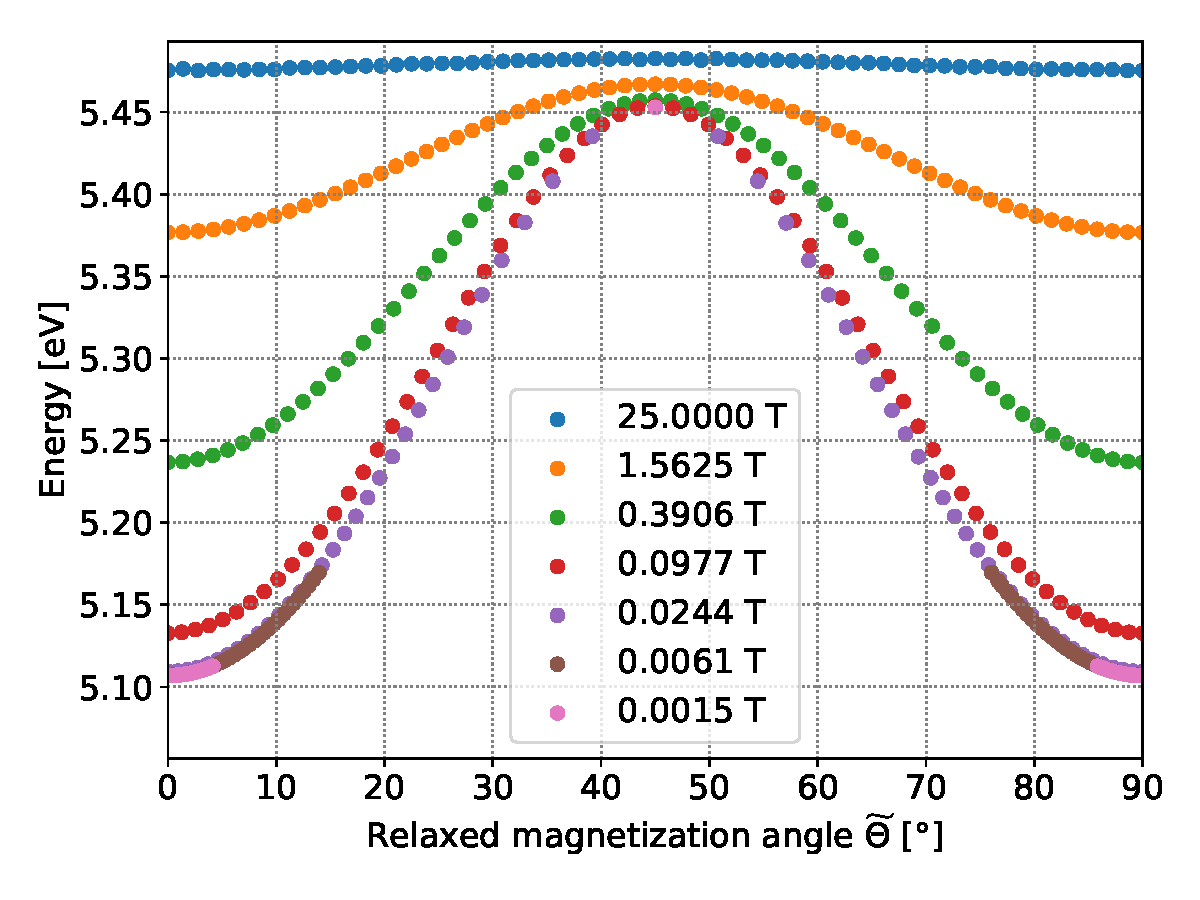
\includegraphics[width=0.9\textwidth]{Figures/biaxial_island/BarrierLandscape/Plus_65_B25-0.001-div4_a128Pi_plotOptimized.pdf}
    \caption{Energy landscape between \SIrange{0}{90}{\degree} for various external magnetic field magnitudes $\abs{\vb{B_{ext}}}$. The external field angle was varied uniformly from \SIrange{0}{90}{\degree} in 64 steps.}
    \label{fig:barrierLandscape-sweepBext}
\end{figure}

Interesting findings:

- Firstly, at very high magnetic fields, the energy landscape is nearly flat as explained earlier.~\cite{Nonmonotonic_reversal}

- Secondly, at an angle of exactly \SI{45}{\degree}, the magnetization remains at the maximum of the energy landscape, which is an unstable equilibrium.

- Thirdly, for lower and lower magnetic field values, the situations for angles very close to \SI{45}{\degree}, the magnetization relaxes to an angle closer to that of the energy minimum. This is to be expected, because lower magnetic fields will have more difficulty keeping the magnetization pointed in the same direction, against the anisotropy.

- Fourthly or finally idk, for lower magnetic fields the energy barrier lowers until it reaches a limit value. This is because high external magnetic fields prevent the relaxation of the edges of the geometry, instead keeping them pointed in roughly the same direction. It is the relaxation of the magnetization angle in a non-uniform way which causes the anisotropy, so forcing the magnetization in a certain direction (like with a high external field) will prevent this from happening, thus increasing the energy and lowering the fictional variant of the energy barrier.

\paragraph{Energy barrier as function of roundness}

\paragraph{Energy barrier as function of overall size}

\paragraph{Numerical error: influence of cell size on energy barrier}
When performing longer simulations, it is advantageous to use as large a cell size as possible, to minimize the total amount of cells in the simulation. Increasing the size of the cells does however also increase the numerical error originating from the discretization of the grid. The size of this numerical error was examined by determining the energy barrier for different shapes (varying roundness and overall size) and for different cell sizes of \SI{4}{\nano\metre}, \SI{2}{\nano\metre} and \SI{1}{\nano\metre}. The results of this calculation are shown in \cref{fig:barrier-cell_size}.
\begin{figure}
     \centering
     \begin{subfigure}[b]{0.75\textwidth}
         \centering
         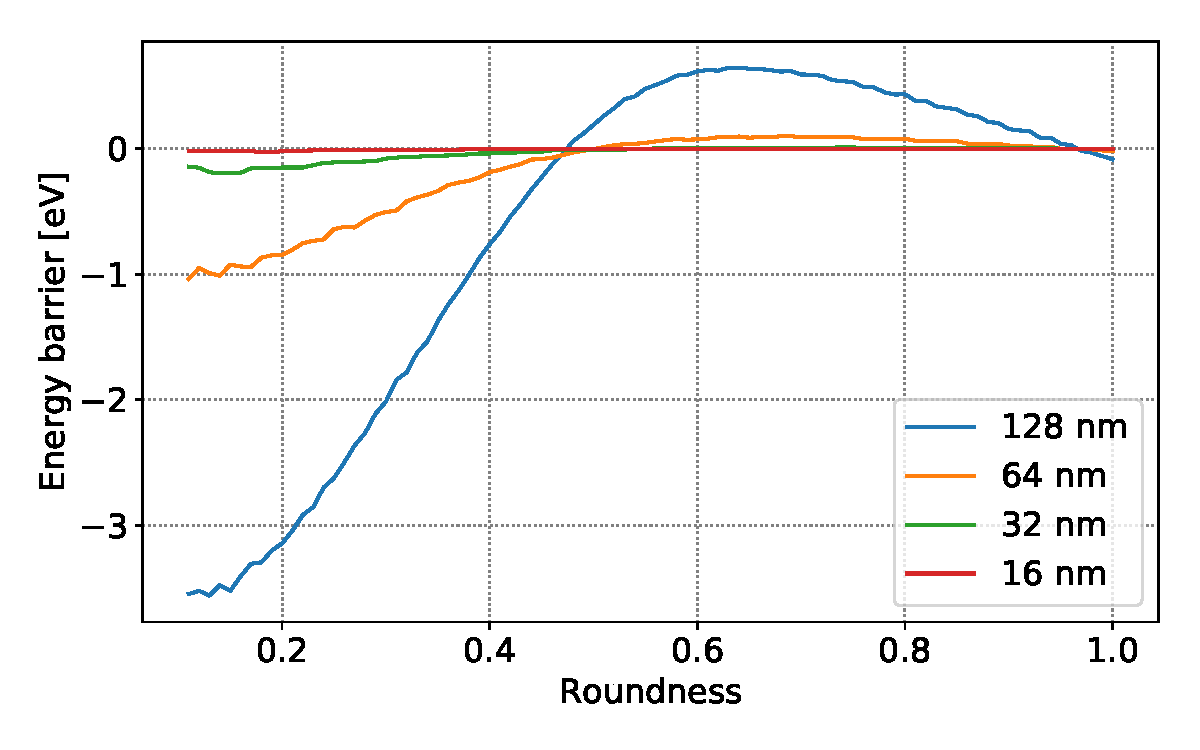
\includegraphics[width=\textwidth]{Figures/biaxial_island/Barrier/Plus_16-128_0.1-1_aPi4_B0.001_cell1nm.pdf}
         \caption{\SI{1}{\nano\metre}}
         \label{fig:barrier-cell_size-1nm}
     \end{subfigure}
     \hfill
     \begin{subfigure}[b]{0.75\textwidth}
         \centering
         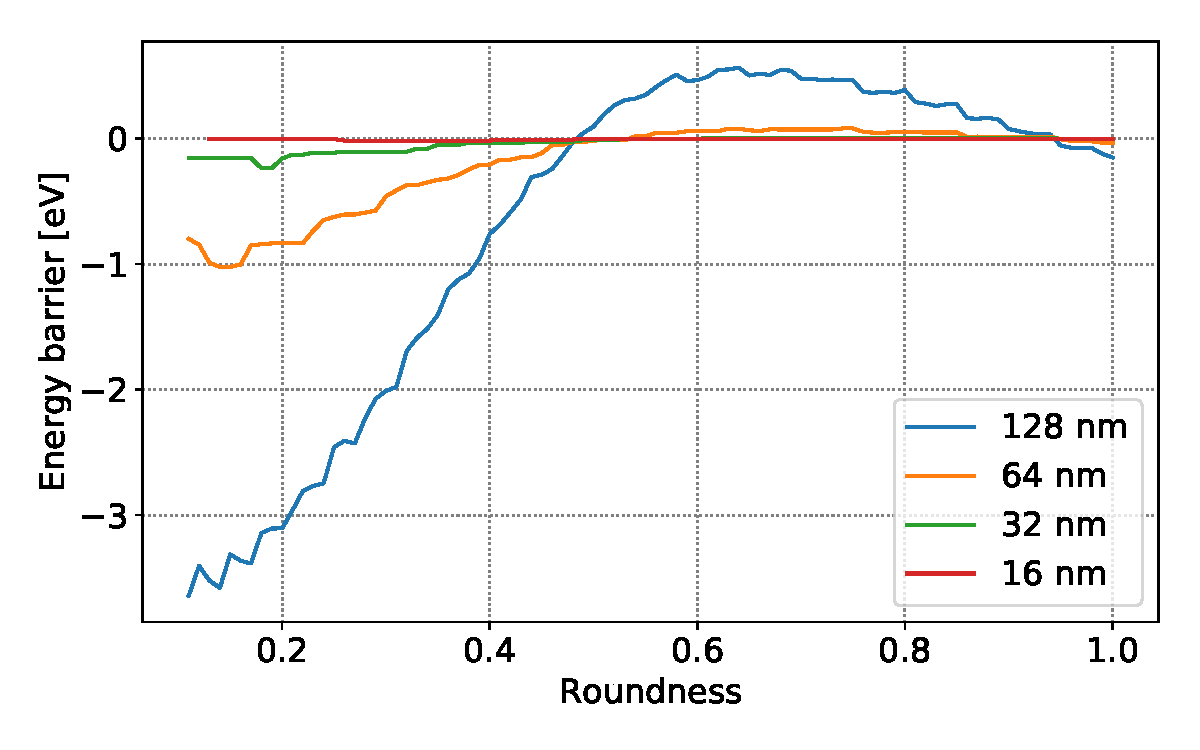
\includegraphics[width=\textwidth]{Figures/biaxial_island/Barrier/Plus_16-128_0.1-1_aPi4_B0.001_cell2nm.pdf}
         \caption{\SI{2}{\nano\metre}}
         \label{fig:barrier-cell_size-2nm}
     \end{subfigure}
     \hfill
     \begin{subfigure}[b]{0.75\textwidth}
         \centering
         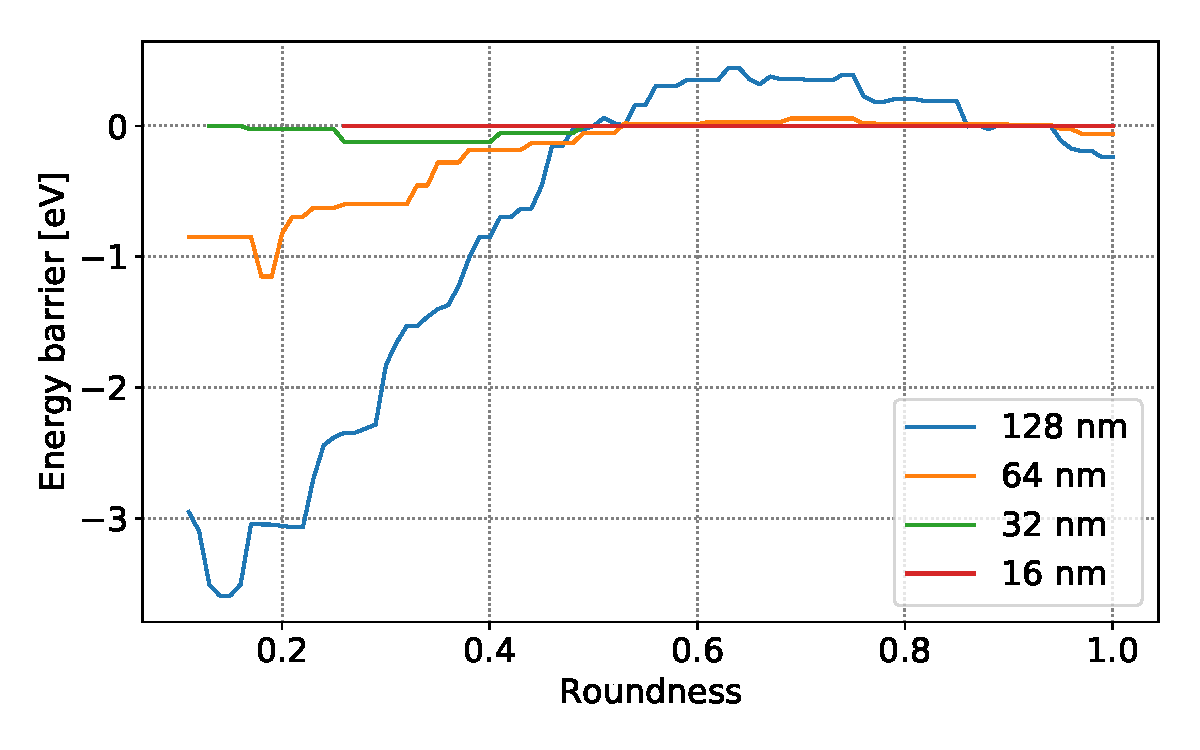
\includegraphics[width=\textwidth]{Figures/biaxial_island/Barrier/Plus_16-128_0.1-1_aPi4_B0.001_cell4nm.pdf}
         \caption{\SI{4}{\nano\metre}}
         \label{fig:barrier-cell_size-4nm}
     \end{subfigure}
        \caption{Energy barrier for different cell sizes. The legend represents the length of the long axis of the ellipses.}
        \label{fig:barrier-cell_size}
\end{figure}
The figure obtained with cells of \SI{1}{\nano\metre} is quite smooth, so it is justified that this size was used in the previous paragraphs. For \SI{2}{\nano\metre} cells, the curve becomes rougher, but the overall shape remains very similar to that of \SI{1}{\nano\metre} cells. Cells of \SI{4}{\nano\metre}, however, yield a very rough and almost stair-like energy landscape, which clearly indicates that this size is too large. \par
It may also be noted that for the \SI{4}{\nano\metre} cells, there are no values for the lowest roundnesses for long ellipse axes of \SI{16}{\nano\metre} or \SI{32}{\nano\metre}, because for these situations the short axis is smaller than the grid size, which yields an empty simulation geometry and thus no results. \par
Everything taken into account, it seems that the optimal compromise between simulation speed and accuracy, is a \SI{2}{\nano\metre} cell size, which will be used to perform longer simulations. For the 65x100nm geometry, a \SI{4}{\nano\metre} cell size is probably still acceptable since the energy barrier is similar, and since this will result in a 4x speed increase this will be used. For the perfectly round situation, the difference is very large so it is instructive to use \SI{2}{\nano\metre} or even \SI{1}{\nano\metre}.




% FROM HERE ON THINGS ARE NOT VERY STRUCTURED
\subsection{Random thermal switching}
\subsubsection{Preparation}
\textbf{Step 1: find energy barrier} \\
The procedure used is to set both $m$ and $B_{ext}$ at a certain angle and then \code{minimize()}. Both the magnetic field $B_{ext}$ and the angle $\theta$ are then varied, with $B_{ext}$ going from very high to very low values, and $\theta=0\dots\pi/2$ in steps of $\pi/4$. One could increase the amount of $\theta$-steps, but it is observed that an angle of $\pi/4$ remains magnetized at that angle regardless of the external field, at the very least until $B_{ext} = \SI{0.00153}{\tesla}$. It is however an unstable equilibrium and any slight deviation from this angle will quickly relax to either \SI{0}{\degree} or \SI{90}{\degree} at low fields.
One could even omit the part where theta goes from $\pi/4$ to $\pi/2$ due to symmetry reasons.
All of $\theta = k\frac{\pi}{4} , k\in\mathbb{Z}$ are stable.
At high fields everything is stable and just uniform, which makes the energy landscape flat.

\textbf{Step 2: random switching over \SI{100}{\nano\second}} \\
In GYP-18~\cite{GYP-18} the formula
\begin{equation}
    t_i = -\frac{1}{f_0} \exp(\frac{\Delta E_i}{k_B T}) \ln(1-P_i)
\end{equation}
appears, with $f_0 = \SI{e12}{\hertz}$ attempt frequency, and $P_i$ random between 0 and 1. The average value of $-\ln(1-P_i)$ is then $\ln(4) \approx 1.4$.

To get an average $t_i = \SI{100}{\nano\second}$ at $T=\SI{300}{\kelvin}$, one should therefore have
\begin{equation}
    \Delta E_i = k_B T \ln(\frac{f_0 t_i}{\ln(4)}) = 11.19 k_B T = \SI{0.310}{\electronvolt} \mathrm{.}
\end{equation}
The barrier height of a \SI{65}{\nano\metre} elliptic plus-sign geometry is \SI{0.346}{\electronvolt}.
Idea: perhaps attempt frequency is the sinusoidal pattern in the long simulations, with period of about \SI{0.5}{\nano\second}. Observation: This worked with the previous method where $B_{ext}$ was not varied, but with the new (correct) method the $f_0 = \SI{e12}{\hertz}$ works very well again.
Also there is another formula in mumax3~\cite{MuMax3} for uniaxial anisotropy.

Observation: with a barrier height approximately equal to $\SI{0.346}{\electronvolt}$, a switching speed of about \SI{100}{\nano\second} is observed.

Question: should $\alpha$ be 0.1 always, i guess this is just a case of ``0.1 works so we use 0.1''
Answer: it's better to use 0.01

\subsubsection{Results}
Step 1: find energy barrier \\
With perfectly circular geometry (i.e. \\
\code{geometry := Ellipse(100e-9, 100e-9)} \\
\code{geometry = geometry.Add(Ellipse(100e-9, 100e-9).RotZ(Pi/2))}) \\
there is still shape anisotropy, but with opposite sign (what are maxima in actual plus-figures are now minima)

Findings (for \SI{100}{\nano\metre} long axis ellipse plus-sign):
at \SI{45}{\nano\metre} the preferred directions switch from the axes (\SI{0}{\degree}) to in between the axes (\SI{45}{\degree}),
at \SI{65}{\nano\metre} the anisotropy with preferred \SI{0}{\degree} direction is the strongest

After running for \SI{1}{\micro\second} at \SI{300}{\kelvin}, with shape \SI{65}{\nano\metre} by \SI{100}{\nano\metre} ellipses in plus shape, the following angles were observed (\cref{fig:biaxial_island:1microsecond_300K_alpha0.1}):
\begin{figure}
    \centering
    \includegraphics[width=1.0\columnwidth]{Figures/biaxial_island/table_1µs_alpha0.1_300K.png}
    \caption{\SI{1}{\micro\second} at \SI{300}{\kelvin}, with $\alpha=0.1$.}
    \label{fig:biaxial_island:1microsecond_300K_alpha0.1}
\end{figure}
\begin{figure}
    \centering
    \includegraphics[width=1.0\columnwidth]{Figures/biaxial_island/table_1µs_alpha0.01_300K.png}
    \caption{\SI{1}{\micro\second} at \SI{300}{\kelvin}, with $\alpha=0.01$.}
    \label{fig:biaxial_island:1microsecond_300K_alpha0.01}
\end{figure}


\newpage
\bibliographystyle{IEEEtran}
\bibliography{bibliography/bibliography.bib}


\end{document}
